\documentclass[12pt]{article}
\usepackage[margin=2.5cm]{geometry}
\usepackage{enumerate}
\usepackage{amsfonts}
\usepackage{amsmath}
\usepackage{fancyhdr}
\usepackage{amsmath}
\usepackage{amssymb}
\usepackage{amsthm}
\usepackage{mdframed}
\usepackage{graphicx}
\usepackage{subcaption}
\usepackage{adjustbox}
\usepackage{listings}
\usepackage{xcolor}
\usepackage{booktabs}
\usepackage[utf]{kotex}
\usepackage{hyperref}

\definecolor{codegreen}{rgb}{0,0.6,0}
\definecolor{codegray}{rgb}{0.5,0.5,0.5}
\definecolor{codepurple}{rgb}{0.58,0,0.82}
\definecolor{backcolour}{rgb}{0.95,0.95,0.92}

\lstdefinestyle{mystyle}{
    backgroundcolor=\color{backcolour},
    commentstyle=\color{codegreen},
    keywordstyle=\color{magenta},
    numberstyle=\tiny\color{codegray},
    stringstyle=\color{codepurple},
    basicstyle=\ttfamily\footnotesize,
    breakatwhitespace=false,
    breaklines=true,
    captionpos=b,
    keepspaces=true,
    numbers=left,
    numbersep=5pt,
    showspaces=false,
    showstringspaces=false,
    showtabs=false,
    tabsize=1
}

\lstset{style=mystyle}

\pagestyle{fancy}
\renewcommand{\headrulewidth}{0.4pt}
\lhead{Team Treehouse}
\rhead{Modifying Data with SQL Part 1 Notes}

\begin{document}
\title{Modifying Data with SQL Part 1 Notes}
\author{Team Treehouse}
\maketitle

\bigskip

\section{Introduction to CRUD}

\bigskip

\section{Adding a Row to a Table}

\bigskip

\begin{itemize}
    \item Adding rows of information into a table (in the order of columns)
    \begin{itemize}
        \item \textbf{Syntax:} INSERT INTO \textit{table name} VALUES (\textit{value 1}, \textit{value 2}, ...);

    \begin{lstlisting}[language=SQL]
    INSERT INTO users VALUES  (1, "chalkers", "Andrew", "Chalkley");


    INSERT INTO users VALUES  (2, "ScRiPtKiDdIe", "Kenneth", "Love");


    INSERT INTO movies VALUES (3, "Starman", "Science Fiction", 1984);


    INSERT INTO movies VALUES (4, "Moulin Rouge!", "Musical", 2001);
    \end{lstlisting}

    \end{itemize}

    \item Adding rows of information into a table (independent of the order of columns)
    \begin{itemize}
        \item \textbf{Syntax:} INSERT INTO \textit{table name} (\textit{column name 1}, \textit{column name 2}) VALUES (\textit{value 1}, \textit{value 2});
        \item \textbf{Syntax \# 2:} INSERT INTO \textit{table name} (\textit{column name 2}, \textit{column name 1}) VALUES (\textit{value 2}, \textit{value 1});

    \begin{lstlisting}[language=SQL]
    INSERT INTO users (username, first_name, last_name) VALUES ("chalkers", "Andrew", "Chalkley");


    INSERT INTO users (first_name, last_name, username) VALUES  ("Kenneth", "Love", "ScRiPtKiDdIe");


    INSERT INTO movies (title, genre, year_released) VALUES ("Starman", "Science Fiction", 1984);


    INSERT INTO movies (title, year_released, genre) VALUES ("Moulin Rouge!", 2001,  "Musical");
    \end{lstlisting}

    \end{itemize}
\end{itemize}

\bigskip

\section{Adding Multiple Rows to a Table}

\bigskip

\begin{itemize}
    \item Adding multiple rows rows of information into a table (in the order of columns)
    \begin{itemize}
        \item \textbf{Syntax:}

        \bigskip

    \begin{lstlisting}[language=SQL]

    \textit{INSERT INTO <table name> (<column name 1>, <column name 2>, ...)}
    VALUES
            (<value name 1>, <value name 2>, ...),
            (<value name 1>, <value name 2>, ...),
            (<value name 1>, <value name 2>, ...);
    \end{lstlisting}

    \begin{lstlisting}[language=SQL]
    INSERT INTO users (username, first_name, last_name)
        VALUES
                      ("chalkers", "Andrew", "Chalkley"),
                      ("ScRiPtKiDdIe", "Kenneth", "Love");


    INSERT INTO movies (title, genre, year_released)
         VALUES
                       ("Starman", "Science Fiction", 1984),
                       ("Moulin Rouge!", "Musical", 2001);
    \end{lstlisting}

    \end{itemize}
\end{itemize}

\bigskip

\section{Exercise 1}

\bigskip

\begin{itemize}
    \item Solution included in \textit{exercise\_1.sql}
\end{itemize}

\bigskip

\section{Review and Practice}

\bigskip

\section{Quiz 1}

\bigskip


\begin{enumerate}[1.]
    \item

    What character should you replace the ? with to create a valid INSERT
    statement?

    \bigskip

    \begin{lstlisting}[language=SQL]
    INSERT INTO awesome_people (first_name, last_name) VALUES ("Grace", "Hopper")? ("Ada", "Lovelace");
    \end{lstlisting}

    \begin{enumerate}[A.]
        \item ,
        \item "
        \item ;
    \end{enumerate}

    \bigskip

    \textbf{Answer:} A

    \item

    \begin{center}
    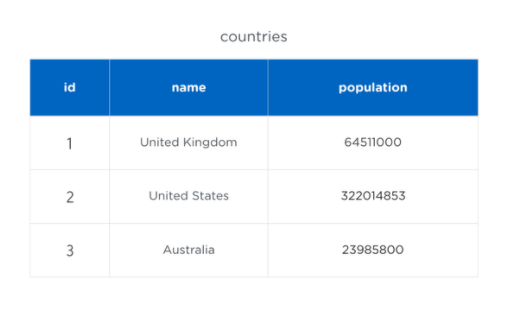
\includegraphics[width=0.8 \linewidth]{images/part_1_notes_1.png}
    \end{center}

    Please fill in the correct answer in each blank provided below.

    \bigskip

    Given the database table imaged above, how would you complete this INSERT statement.

    \bigskip

    \begin{lstlisting}[language=SQL]
    INSERT INTO countries (population, ____) VALUES (4596700, "New Zealand");
    \end{lstlisting}

    \bigskip

    \textbf{Answer:} name

    \item

    What does the acronym CRUD stand for?

    \bigskip

    \begin{enumerate}[A.]
        \item Create, Read, Update and Delete
        \item Curate, Retrieve, Update and Delete
        \item Create, Render, Update and Duplicate
    \end{enumerate}

    \bigskip

    \textbf{Answer:} A

    \item

    Please fill in the correct answer in each blank provided below.

    \bigskip

    \begin{lstlisting}[language=SQL]
    INSERT \_\_\_\_\_  tv_shows (show, network) \_\_\_\_\_  ("Super Girl", "CBS");
    \end{lstlisting}

    \bigskip

    \textbf{Answer:} INTO, VALUES

    \item

    How many rows will this statement insert in to the cars table?

    \bigskip

    \begin{lstlisting}[language=SQL]
    INSERT INTO cars (make, model) VALUES ("Fiat", "Fiat 500"),
        ("Fiat", "Fiat Multipla"),
        ("Cadillac", "Cadillac Fleetwood"),
        ("Cadillac", "Cadillac Eldorado");
    \end{lstlisting}

    \bigskip

    \begin{enumerate}[A.]
        \item 5
        \item 4
        \item 3
    \end{enumerate}

    \bigskip

    \textbf{Answer:} B
\end{enumerate}

\end{document}